\documentclass[tocnopagenum]{thesis-ekf}
%a4paper, 12pt, 1.5-es sortávolság, margók
\PassOptionsToPackage{defaults=hu-min}{magyar.ldf}
\usepackage[magyar]{babel}
\usepackage[T1]{fontenc}
\usepackage[utf8]{inputenc}
\usepackage{mathtools,amssymb,amsthm,pdfpages}
\footnotestyle{rule=fourth}
\usepackage{comment}
\usepackage{enumitem}
\usepackage{booktabs}


\newtheorem{tetel}{Tétel}[chapter]
\theoremstyle{definition}
\newtheorem{definicio}[tetel]{Definíció}
\theoremstyle{remark}
\newtheorem{megjegyzes}[tetel]{Megjegyzés}

\begin{document}
	\institute{Matematikai és Informatikai Intézet}
	\title{Interfész megoldások imperatív és OOP nyelvek közötti kapcsolattartásra}
	\author{Nagy-Tóth Bence\\Szak: Programtervező informatikus BSc\\Specializáció: Szoftverfejlesztő informatikus}
	\supervisor{Dr. Király Roland\\beosztás}
	\city{Eger}
	\date{2022}
	\maketitle
	\tableofcontents
	
	\chapter*{Bevezetés}
	\addcontentsline{toc}{chapter}{Bevezetés}
	Az ember kognitív képességeinek fejlesztésére mindig is szükség volt, van, és lesz is a jövőben. Ez a megállapításom különösen beigazolódni látszik egy COVID-világjárvány utáni időszakban, amikor is sorra jelennek meg olyan jelentések \emph{TODO referencia erre} \cite{brain1}
	, amelyek azt támasztják alá, hogy a lezárások ideje alatt nőtt a különböző mentális betegségek (pl. demencia, \emph{TODO példák}
	) kialakulásának kockázata. Nem beszélve arról, hogy a digitális eszközök használata számtalan alkalommal hosszas órákon keresztül képes lekötni a figyelmünket, ezért bizonyos külső ingerekre egyre lassabban, egyre kisebb amplitúdóval (nagyobb közömbösséggel) vagyunk képesek reagálni.
	\chapter{Programozási nyelvekről általában}
	\section{A programozási nyelvek formális nyelvek?}
	\begin{definicio}
		Legyen $\mathbb{A} = \{a_1, a_2, ... a_n\}$ véges, nemüres ($ \mathbb{A} \neq \emptyset$) halmaz, ezt a nyelv ábécéjének, elemeit betűknek vagy jeleknek nevezzük. $\mathbb{A}$ halmaz elemeiből képezzük annak hatványait, ekkor 
		\begin{enumerate}
			\item $\mathbb{A} ^ {0}$ az üres szó ($\epsilon$) egyelemű halmazát, 
			\item $\mathbb{A} ^ {1} $ az egybetűs szavak (\,$\mathbb{A}^{1}\subseteq\mathbb{A}\wedge\mathbb{A}\subseteq\mathbb{A}^{1} \iff \mathbb{A}^{1}=\mathbb{A}$\,), 
			\item $\mathbb{A}^{2}$ a kétbetűs szavak, 
			\item $\mathbb{A}^{n}$ az $n$ hosszú szavak halmazát jelenti és így tovább.
		\end{enumerate}
	Jelölje $A^{*}=A^{0}\ \cup\ A^{1}\ \cup\ A^{2}\ \cup\ \dots\ \cup\  A^{n}$ az ábécé elemeiből képzett véges szavak vagy más néven jelsorozatok halmazát (ezt az $\mathbb{A}$ ábécé feletti univerzumnak hívjuk). Ekkor  $\mathbb{A}$-ból kirakható szavak $\mathbb{A}^{*}$ halmazának egy részhalmazát \textbf{formális nyelvnek} nevezzük. Szokásos még az $\mathbb{A}$ ábécé feletti formális nyelv megnevezés is. A hatványok a halmaz önmagával vett \emph{Descartes-szorzatait} jelentik.
	\cite{formnyelvek}
	\end{definicio}
	
	Fő különbségek formális és természetes nyelvek között:
	\begin{itemize}
		\item A formális nyelveket egy dedikált célra hozzuk létre, ezeket általában nem használjuk interperszonális (emberek közötti) kommunikációra. Ezzel szemben egy természetes nyelv (például az angol) egy emberi közösség aktuális és a múltban használt jelkészletét rendszerezi.\\
		A C++ programozási nyelv például azért jöhetett létre Bjarne Stroustrup dán szoftverfejlesztő jóvoltából, mert a C - procedurális nyelv lévén - nem tette lehetővé többek között a tisztább objektum-orientált programozást, a memóriacímek helyett a biztonságosabb referenciák használatát. \cite{cpplang1}
		\item A formális nyelvek kulcsszavakból állnak. A természetes nyelvek több építőelemből tevődnek össze: fonémák (hangok, betűk), morfémák (szótövek, toldalékok), szavak, mondatok, bekezdések, szövegek.
		\item A természetes nyelvek fejlődhetnek spontán, emberi generációról generációra valamint tudatos módon (például nyelvújítás) egyaránt. A formális nyelvek alakulását egy tervezési fázis előzi meg, ekkor a nyelv szabályrendszerét lefektetik, tehát csak és kizárólag tudatos, mesterséges beavatkozással lehet megreformálni őket.
	\end{itemize} \cite{langvid1} \cite{langvid2}

	A fentiekből következően minden programozási nyelv formális nyelvnek számít. 
	\section{Jelenleg népszerű programozási nyelvek}
	2022-ben a legnépszerűbb programozási nyelveknek számítanak (a teljesség igénye nélkül):
	\begin{enumerate}
		\item JavaScript
		\begin{itemize}
			\item 1995, Brendan Eich fejlesztette a webböngészési funkcionalitások kibővítése végett.
			\item web-, játék-, valamint mobilfejlesztésre egyaránt használják
			\item webszerverként is tud funkcionálni (Node.js)
		\end{itemize}
		\item Python
		\begin{itemize}
			\item 1991, Guido Van Rossum tervezte annak érdekében, hogy olvashatóbb és nagyobb kifejezőerővel rendelkező kódok készülhessenek, a szintaktikai szabályok helyett a kód működésére tudjanak a programozók koncentrálni
			\item backend-fejlesztés
			\item automatizálás
			\item web scraping\footnote{Információgyűjtés eszköze, amely lehetővé teszi, hogy automatizált módon (kód segítségével) bizonyos weboldalakról tetszőleges adatokat (például posztokat, közelgő eseményeket) letölteni.}
			\item Data Science\footnote{Az informatika, a matematikai statisztika és az üzleti elemzés metszetében álló tudományág, amely adatok összegyűjtésével, ezek elemzésével foglalkozik annak érdekében, hogy a vállalatok jobb üzleti döntéseket tudjanak meghozni ezek segítségével. \hyperref{https://qr.ae/pvlYmQ}{}{}{Forrás}}
		\end{itemize}
		\item HTML
		\begin{itemize}
			\item webdokumentumok kezelése: JSON, XML, SVG
			\item weboldalak statikus (állandó) részeinek fejlesztése
		\end{itemize}
		\item CSS 
		\begin{itemize}
			\item weboldalak formatervét, kinézetét, stílusát alakítja ki
			\item HTML mellett hívják segítségül
		\end{itemize}
		\item Java
		\begin{itemize}
			\item 1995, Sun Microsystems fejlesztése, alapötlet: olyan eszközök vezérlése, amelyek elférnek egy kézben
			\item E-kereskedelem
			\item Financial Technology: pénzintézetekkel, tőzsdékkel, számlázással kapcsolatos szoftvereket jellemzően ezen a nyelven fejlesztik
			\item a megírt kódok futtathatóak különösebb átalakítás nélkül az elterjedtebb operációs rendszereken (a kód hordozható, platformfüggetlen)\footnote{Ez azért lehetséges, mivel .exe fájl helyett egy átmeneti .class állomány (bytecode) készül, amit egy virtuális gép (Java Virtual Machine) tolmácsolja (interpretálja) gépi kódként a számítógépünknek \hyperref{https://www.upgrad.com/blog/why-is-java-platform-independent-language/}{}{}{Forrás}}
		\end{itemize}
		\item SQL
		\begin{itemize}
			\item 1972, Donald D. Chamberlin és Raymond F. Boyce az IBM alkalmazásában, adattáblák egyszerűbb kezelésére
			\item adatbázisok kezelése, karbantartása
			\item Data Science
		\end{itemize}
		\item Go
		\begin{itemize}
			\item 2009, a Google fejlesztői alakították ki, hogy megoldják a hatalmas szoftverrendszerekkel kapcsolatos problémákat
			\item rendszerek, hálózatok programozása
			\item hang- és videószerkesztés
			\item Big Data\footnote{Az informatika egyik tudományága, amely tömérdek mennyiségű, hagyományos számítógéppel nehezen kezelhető adatok tárolásával és feldolgozásával, ezek elemzésével foglalkozik.\hyperref{{https://www.youtube.com/watch?v=bAyrObl7TYE}}{}{}{Forrás}}
		\end{itemize}
		\item C
		\begin{itemize}
			\item 1970-es években Ken Thompson és Dennis Ritchie jóvoltából, Assembly-nél magasabb szintű (természetes nyelvezethez közelebb álló) nyelv kialakítása volt a célja
			\item beágyazott rendszerek illesztőprogramjai, vezérlőkódjai
			\item operációs rendszerek fejlesztése
			\item 3D videók szerkesztése
			\item alacsonyabb szintű a fentebb felsoroltaknál, ezért könnyebb optimalizálni memória és futásidő szempontjából
			\cite{clang1}
		\end{itemize}
	\end{enumerate}\cite{proglanguages1}\cite{proglanguages2}
	
	\chapter{Marshalling}
	\section{Milyen adatszerkezeteink vannak?}
	A programozási nyelvek szintaktikában ugyan eltérnek egymástól, amikor viszont adatok tárolásáról van szó, egy dologban egyetértenek: típusokra szükség van. Mit jelent az, hogy egy változót például bool típusúként definiálunk? Az adat típusa meghatározza, hogy
	\begin{itemize}
		\item mekkora memóriaterületet\footnote{mivel a byte számít a legkisebb megcímezhető memóriaegységnek, ezért ennek mértékegysége alapértelmezetten byte-ban értendő} kell számára lefoglalni
		\item a számítások folyamán hogyan kell őt értelmezni\\(például ha másik változónak értékül adjuk, hány bitet kell másolni)
		\item továbbá milyen műveletek végezhetőek vele\\(például egész típusú változókon értelmezhetjük a szorzás műveletét, szövegeknél ezt már nem tehetjük meg).
	\end{itemize} \cite{adatszerkezetek_88}
	\section{Használt adatszerkezetek}
	Ahogy említettem, a programozási nyelvek döntő része típusos, ezenfelül kisebb-nagyobb különbséggel hasonló adatszerkezeteket értelmez.
	\begin{enumerate}[label=\alph*)]
		\item \emph{elemi adattípusok}: Olyan típusok, amiket nem tudunk további részekre bontani, csak egyben értelmezhetjük őket. Ilyen például a \verb*|double| lebegőpontos típus, amely 8 byte-on képes lebegőpontos számot ábrázolni. Igaz, hogy csak az első byte-ra van mutatónk, de nincs értelme további byte-okra darabolni, és megnézni az értékeket, mivel egyben értelmezendő, a műveleteket 4 byte-on fogjuk tudni vele végezni. Primitív adattípusoknak is nevezzük őket.\\
		Vegyük például a C\# programozási nyelvet, milyen elemi típusai vannak?
			\begin{enumerate}
				\item egész:
				\begin{tabular}{ccc}
					Előjeles változat & Előjel nélküli változat & Méret (Byte) \\
					sbyte & byte & 1 \\
					short & ushort & 2 \\
					int & uint & 4 \\
					long & ulong & 8 \\
				\end{tabular}
				\item lebegőpontos:
				\begin{tabular}{cc}
					Név & Méret (Byte) \\
					float & 4 \\
					double & 8
				\end{tabular}
				\item logikai: 
				\begin{tabular}{cc}
					bool & 1 Byte
				\end{tabular}
				\item karakteres: 
				\begin{tabular}{cc}
					char & kódolástól függ\footnote{ASCII kódolás esetén 1 karakter 7, míg UTF-8 kódolás esetében 8 biten}
				\end{tabular}
			\end{enumerate}
	\item \emph{összetett adattípusok}: Az összetett adattípusok elemi típusokra szedhetők szét, vagyis primitív és/vagy további összetett típusú változókból épülnek fel, ezeket mezőknek hívjuk. Az összetett adattípusú változó memóriaterülete kiszámítható az adattagok összegével.\\
	C\#-ban a \verb*|struct| és a \verb*|class| kulcsszavakkal tudunk összetett típusokat definiálni.
	\end{enumerate}
	\section{Mi a helyzet az algoritmusokkal?}
	Adatokat tudunk tárolni, de nyilvánvalóan azért, mert tervünk van velük, valamit szeretnénk velük kezdeni. Az adatszerkezeteken végzett véges elemi lépéssorozatot algoritmusnak nevezzük. Az adatszerkezetek algoritmusok nélkül olyanok, mint a matematikai műveletek operátorok (összeadás, kivonás, stb.) nélkül, végül -- ha már említettem a természetes nyelveket--: mint a főnevek igék nélkül.
	\section{Kommunikáció adatszerkezeteken keresztül}
	A Marshalling egy olyan folyamat, amely összetett típusok átalakítására szolgál, hogy egy nyelv adatszerkezetét a másikkal megértessük. Magyar fordításával nem találkoztam ennek a kifejezésnek, de a legjobban talán úgy lehetne megfogalmazni, mint: átrendezés, rendszerezés, tehát befogadhatóvá tesszük az adatszerkezeteinket.
	\par
	A Marshalling sajnos nem minden esetben szolgáltat tökéletes megoldást, szakdolgozati projektünkön keresztül például látni fogjuk, hogy a kód további portolhatósága, újrahasznosíthatósága végett megéri szabványos formátumokon keresztül (pl. JSON-, XML-formátumok) kommunikálni, hogy más felületekre való költöztetés esetén kompatibilitási probléma többé már ne merülhessen fel.
	\section{Mik a stub-ok?}
	A stub-ok hívó (aki csak az implementált metódus fejlécét\footnote{a metódus fejlécét szignatúrának is nevezzük: ez a metódus visszatérési típusát (a void is visszatérési típus!), a függvény nevét, valamint a paraméterlistáját együttesen teszi ki}) és a hívott (ahol a két kód szerződésében lévő publikus/,,meghirdetett''/exportált metódusok -- és még akár továbbiak is -- implementálva vannak) fél között elhelyezkedő mini egységek.
	
	\chapter{Szakdolgozati projektünkről}
	A szakdolgozat mellé készített projektemet Sipos Levente hallgatótársammal fejlesztjük. Ez arról szól, hogy Keresztes Péter tanár úr által Delphi-ben készített metódusokat hívjuk meg C\#-os környezetben. A C\# és Delphi nyelvek összehangolása az én feladatom, a végső termék terveim szerint egy megfelelően dokumentált, jól kitesztelt C\# DLL-állomány lesz, úgynevezett helper-metódusokkal, amelyeket Levente az ő grafikus alkalmazásában tud meghívni.
	\section{Miről is szól a projektünk?}
	Egy mentális egészségfejlesztésre használatos alkalmazást fejlesztésére vállalkoztunk 2022 szeptemberében, amely elméleti alapjait Somodi László futballedző munkásságának köszönhetjük, ezekről titoktartási szerződésünk %ezt betehetnénk ide vagy hivatkozzunk rá
	révén csak nagyon érintőlegesen fogok beszámolni a későbbiekben. A készített alkalmazásunk gyakorlatilag különböző fény- és hangjelzések kibocsátására alkalmas eszközök (több LED-ből felépülő lámpák, nyilak és hangszórók) vezérléséből áll, egy ún. \emph{intelligens szobában} az eredeti tervek szerint 8 eszköz (a készített program azonban tetszőleges, $n$ darabszámú eszköz vezérlésére lett felkészítve) együttes vezérlését kell kezelnünk megadott időközönként (ezeket ütemnek fogjuk nevezni). A program azzal indít, hogy felméri az USB-porton csatlakoztatott, egymással RJ-21 csatlakozókkal sorba kapcsolt eszközöket, őket a típusának megfelelő azonosítóval látja el. Az azonosító meghatározza, hogy egy eszköz milyen típusú. 
	Egy feladatsor több egymást követő ütemből áll, mely a programban azt fogja jelenti, hogy x másodperc késleltetéssel a felmért eszköz tömb elemeinek tulajdonságait (mezőit) a feladatsor aktuális ütemének megfelelően módosítjuk. Mivel minden eszközt együttesen vezérlünk, a program ütemenként az összes eszköz állapotát felül fogja írni, ezért szükségünk van egy olyan állapotra is, ami azt közli az adott eszközzel, hogy éppen semmit ne csináljon (várakozzon). Ez a fényeszközök esetében egyszerűen (0,0,0) RGB-színkód\footnote{Az RGB-színkódolás egy szín leírását három komponens, vörös (\textbf{R}ed), zöld (\textbf{G}reen) és kék (\textbf{B}lue) alapszínek arányától teszi függővé.} közlését, míg hangeszköz esetén egy 0 dB hangerejű tetszőleges frekvenciájú hangjelzés kiküldését fogja jelenteni.
	Somodi László edzővel való együttműködésünk Dr. Király Roland tanár úr segítségével jöhetett létre, akinek múltbéli tapasztalatait és az alkalmazással kapcsolatos ötleteit folyamatos egyeztetések, konzultációk útján tudtuk segítségül hívni.
	\section{Problémák, akadályozó tényezők}
	A következő problémákba ütköztünk eddig:
	
	\section{DLL-függvények bemutatása}
	A következőkben a Keresztes Péter tanár úr által Delphi-ben implementált metódusokat, ezek kezelésének lehetőségeit fogom részletezni.
	Általánosságban elmondható, hogy minden függvény egész típusú értékkel tér vissza, amely érték tájékoztat a lefutás eredményességéről: amennyiben a hívott metódus sikeresen (hiba, kivétel nélkül) lefutott, 0-val tér vissza, ahogy ezt egyébként az operációs rendszerek processzeinél is megszokhattuk. Ettől eltérő értékek az egyes hibatípusokat hivatottak meghatározni a Win32-szabvány\footnote{A Win32-es hibakódok szabványa szerint minden hibakódnak a $0x0000$ (decimálisan: 0) és $0xFFFFFF$ (decimálisan: $16\,777\,215$) közötti tartományban kell lennie.} keretein belül. Ezen hibakódok projektünkre vonatkozó részét az alábbi táblázatban \ref{tab:errcodes} összegyűjtöttem.
	\subsection{DLL megnyitása}
	A program indulásakor elsőként lefutó \verb*|SLDLL_Open| függvényt hívva elkezdhetjük az SLDLL további metódusainak használatát.
	\subsection{Eszközök felmérése}
	\verb*|SLDLL_Felmeres|
	\subsection{Hibakódok}
	\begin{table}[h!]
		\begin{tabular}{|c|c|l|l|}
	\toprule
	Win32-hibakód &                  Hiba címe &                      Hiba jelentése (SLDLL esetén) &                                   Gyakorlati példa \\
	\midrule
	0 &   NO\_ERROR / ERROR\_SUCCESS &                     A függvény sikeresen lefutott. & Program indításakor nem érkezik hibaüzenet (nin... \\
	13 &         ERROR\_INVALID\_DATA & Az azonosító típusjelölő bitpárosa hibás, vagy ... & SLDLL\_SetLampa függvényt hangszóró típusú eszkö... \\
	24 &           ERROR\_BAD\_LENGTH & Hanghossz nem [1;16] intervallumból kap egész é... & SLDLL\_SetHang függvény rosszul lett felparaméte... \\
	71 &        ERROR\_REQ\_NOT\_ACCEP &        Jelenleg fut már egy függvény végrehajtása. & SLDLL\_Felmeres-t hívja meg, miközben az SLDLL\_S... \\
	85 &     ERROR\_ALREADY\_ASSIGNED & Az új azonosító más panelt azonosít, egyedinek ... &                Nem találkoztam még ezzel a hibával \\
	110 &          ERROR\_OPEN\_FAILED &              megadott fájlt nem sikerült megnyitni &                Nem találkoztam még ezzel a hibával \\
	126 &        ERROR\_MOD\_NOT\_FOUND & megadott fájl nem a firmware-re vonatkozó friss... &                Nem találkoztam még ezzel a hibával \\
	1114 &      ERROR\_DLL\_INIT\_FAILED &               Az SLDLL\_Open még nem lett meghívva. & bármely SLDLL-függvényt úgy hívjuk meg, hogy el... \\
	1247 &  ERROR\_ALREADY\_INITIALIZED &                A függvény meghívása már megtörtént &  SLDLL\_Open függvény egymás után 2x való meghívása \\
	1626 &  ERROR\_FUNCTION\_NOT\_CALLED &                   nincs csatlakoztatott USB-eszköz & SLDLL\_Open függvény hívásakor nincsenek csatlak... \\
	egyéb & Windows műveleti hibakódok &                                                NaN &                                                NaN \\
	\bottomrule
\end{tabular}
		\caption{Hibakódok a Win32-szabványból}
		\label{tab:errcodes}
	\end{table}
	
	
	
	
	\cite{errcodes}
	Ezen hibakódokat C\#-ban megfelelő, egyénileg definiált kivételekkel, és sokkal kifejezőbb üzenetekkel váltom fel. 
	\begin{comment}
		Ezek később lesznek hasznosak
		\begin{tetel}
			Tétel szövege.
		\end{tetel}
		
		\begin{proof}
			Bizonyítás szövege.
		\end{proof}
		
		\begin{definicio}
			Definíció szövege.
		\end{definicio}
		
		\begin{megjegyzes}
			Megjegyzés szövege.
		\end{megjegyzes}
	\end{comment}
	
	\chapter*{Összegzés}
	\addcontentsline{toc}{chapter}{Összegzés}
	\verb*|#TODO|: Összefoglalás...
	\bibliographystyle{plain}
	\bibliography{references}
	
	% Aláírt, szkennelt nyilatkozat beillesztése a szakdolgozat végére
	%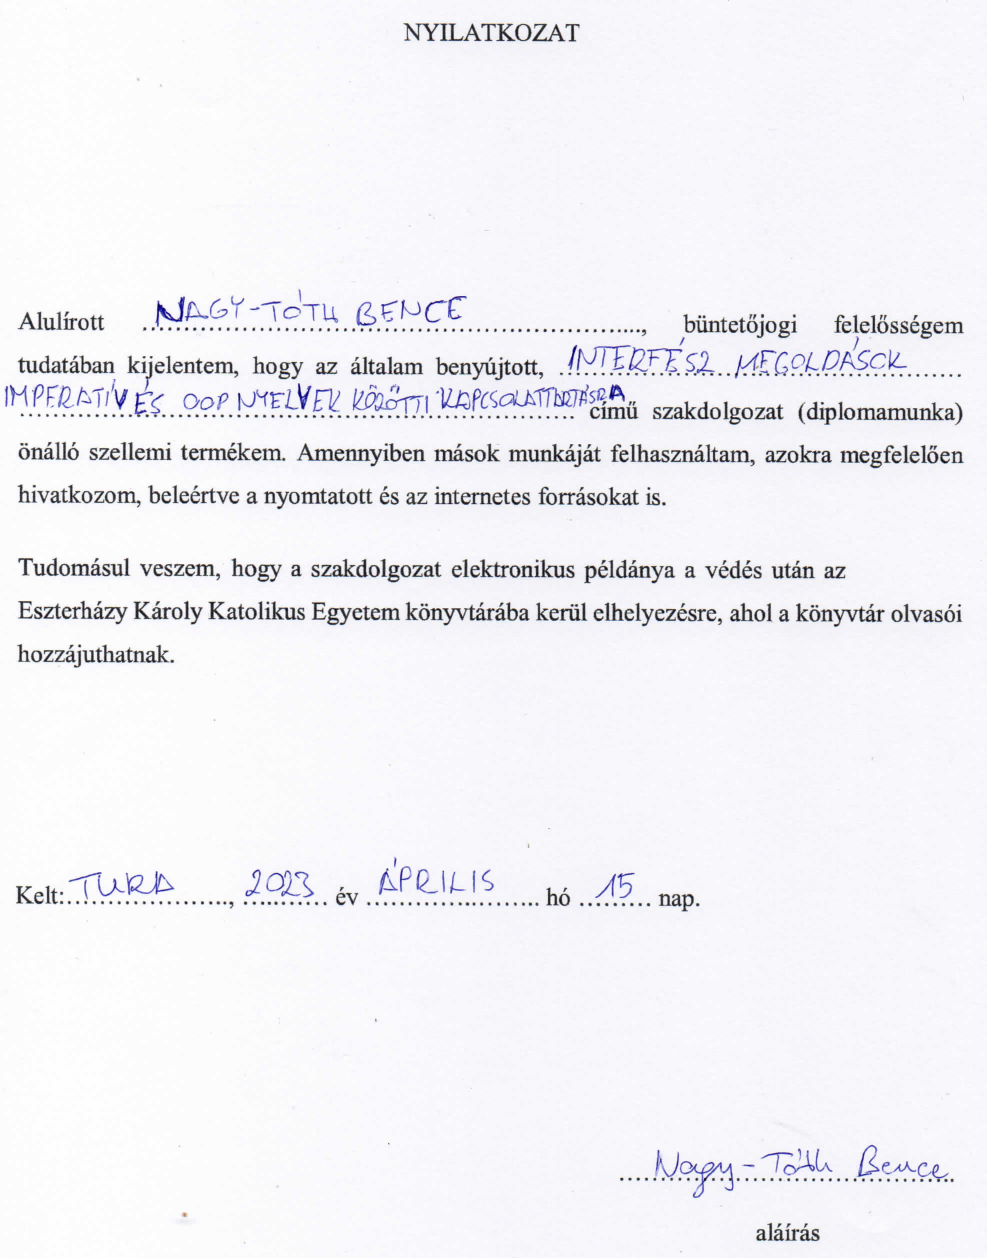
\includepdf{nyilatkozat.pdf}
\end{document}